\section{Multivariate Motif Mining to Disaggregation}
With the advent of modern sensor technologies, 
significant opportunities have emerged to help conserve energy in 
residential and commercial buildings. Moreover, the rapid \emph{urbanization} we are witnessing requires optimized energy distribution. 
Energy disaggregation attempts to 
separate the energy usage 
of each circuit or each electric device in a building 
using only aggregate electricity usage information from 
the whole house meter. 
Usually two-phase or three-phase electric power is 
connected to residential and commercial buildings. 
%Similarly, water disaggregation aims to discover each 
%water use end by only knowing the 
%hot and cold water usage from the whole house water meter.
We tackle energy disaggregation as a multiple-phase data disaggregation problem. 
The aim of this section is to identify electrical devices from 
two phases of aggregated data. 
Unlike previous work which disaggregate devices
from the sum of multiple phases, 
the time series information from each phase and the correlation of a device between/among phases 
are fully used.  
All of this information enables us to characterize more devices. 

%This work makes the following contributions in the field of disaggregation:
%\begin{enumerate}
%\item It can disaggregate aggregate data from multiple phases.
%\item It can separate the continuously variable loads which are mixed in electricity. 
%\item This approach can be used for both electricity disaggregation and water disaggregation.
%\end{enumerate}

\subsection{Disaggregation Formalism}
We propose a semi-supervised approach for disaggregation; i.e.
We assume that we know the on and off events for a short period of time for all devices, %or water end uses, 
and use that information to deduce the power levels, %or water usage, 
or to obtain the startup vectors of every device.

For our purposes, we define the disaggregation problem as follows:
Given $K$-phase aggregated power 
%or $K$ aggregated water consumption time series 
$Y_k=y_1^{(k)}, ..., y_T^{(k)}$, and a set of
power %or water related 
and contextual features, $f=f_1, ..., f_T$ over a period of time T, 
the problem is to estimate the disaggregated power %or water consumption 
of $M$ devices 
$\hat{X_m }= \hat{x}_{1}^{(m)}, ...\hat{x}_{t}^{(m)}, ... \hat{x}_{T}^{(m)}, m\in[1, M]$, 
such that a loss function of the sum of the power %or water consumption 
of the $M$
devices and the sum of the $K$ phases of aggregated power %or water consumption 
is minimized. 
\begin{equation}
\label{eq_powerObj}
\min_{\hat{x}_{t}^{(m)}} \{ \sum_{t=1}^T \mathscr{L}_t(\sum_{m=1}^M \hat{x}_{t}^{(m)}, \sum_{k=1}^Ky_t^{(k)}) \},
\end{equation}
where $\mathscr{L}_t$ is the loss function between 
the sum of $M$ estimated time series at $t$, 
and $y_t^{(k)}$ is the ground truth phase $k$ aggregated power %or water 
feature at time $t$. 
$\mathscr{L}$ is usually the $\mathscr{L}1$-norm $|\sum_{m=1}^M \hat{x}_{t}^{(m)} -\sum_{k=1}^K y_t^{(k)}|$
or the $\mathscr{L}2$-norm $(\sum_{m=1}^M \hat{x}_{t}^{(m)}-\sum_{k=1}^Ky_t^{(k)})^2$.

\subsection{Recursive Multivariate Piecewise Motif Mining}
To solve the problem of separating a multi-dimensional time series into several time series, 
I propose the approach of recursive multivariate piecewise motif mining. 
Motif mining has been well studied in previous work \cite{motif1} and \cite{motif2}. 
Multivariate or multidimensional motif mining is further extended in \cite{minnen2007improving} and \cite{tanaka2005discovery} and \cite{motifgoal}. 

Motif mining is applied to energy disaggregation in \cite{shao2013temporal}, 
in which discrete on/off events are exploited. 
This research enhances previous work by piecewise motif mining, 
where the on/off event is comprised of several consecutive data points, 
i.e. piecewise, other than individual discrete one.
Also, I use multivariate motif mining to make full use of two- or three-phase aggregated data. 

The framework of recursive multivariate piecewise motif mining to energy disaggregation is illustrated in Figure \ref{fig_multivariateMotifming}. 
The input includes multiple-phase aggregated data, such as two-phase data Mains1 and Mains2, 
and the power levels of each device. 
During the whole procedure, I recursively apply piecewise motif mining to two-phases and single phase diffs data.
The first step is to identify electrical devices which draw power from both phases.
Generally these devices consume a large amount of power, such as the water heater indicated by the blue line.
These devices draw equal power or disparate power from both phases synchronously. 
%draws equal power from both phases. 
%By comparing the diffs of these two phases, 
%we discover the same power changes during the on/off events. 
%With multivariate motif mining, 
%we can identify these large power consumption devices. 
Secondly, I remove the power consumption of the devices which draw power from both phases.
This action decreases the noise interference caused by large power consumption 
and increases the possibility to disaggregate more devices with low-power consumption. 
Then we apply piecewise motif mining to single-phase data to separate 
the devices that draw power only from that phase, 
such as the humidifier indicated by the green line. 
\begin{figure}[h]
\centering
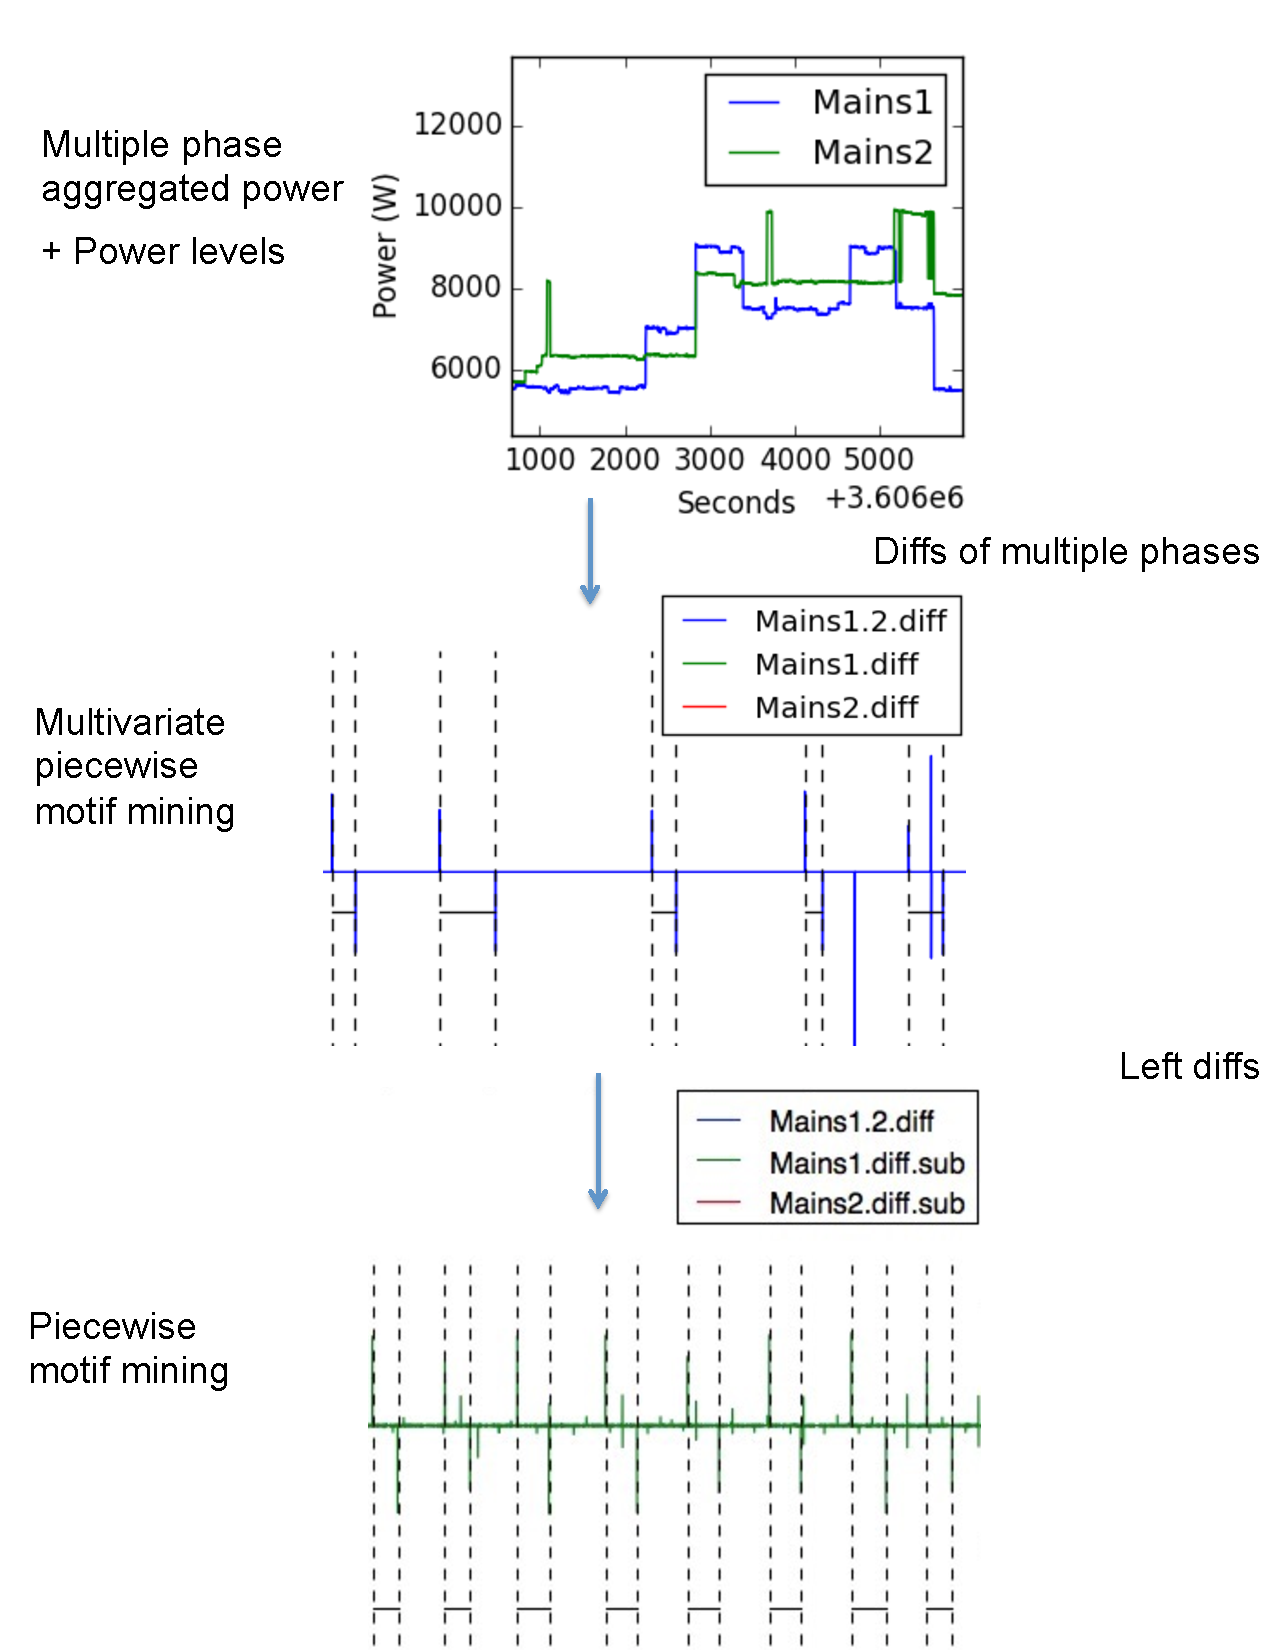
\includegraphics[width=0.5\textwidth]{multidisaggfig/RecursiveMultivariateMotifMining.pdf}
\caption{Recursive Multivariate Motif Mining Approach.}
\label{fig_multivariateMotifming}
\end{figure} 

Generally, multivariate piecewise motif mining is divided into four steps, as shown in Figure \ref{fig_multivariatePiecewiseMotifMining}.
Step 1 is to search for piecewise events from the two-phase or three-phase data.
Step 2 is to encode events from multiple phases. 
Step 3 aims to mine frequent motifs from the encoded events list.
The last step targets to recover devices from mined motifs. 
\begin{figure}[h]
\centering
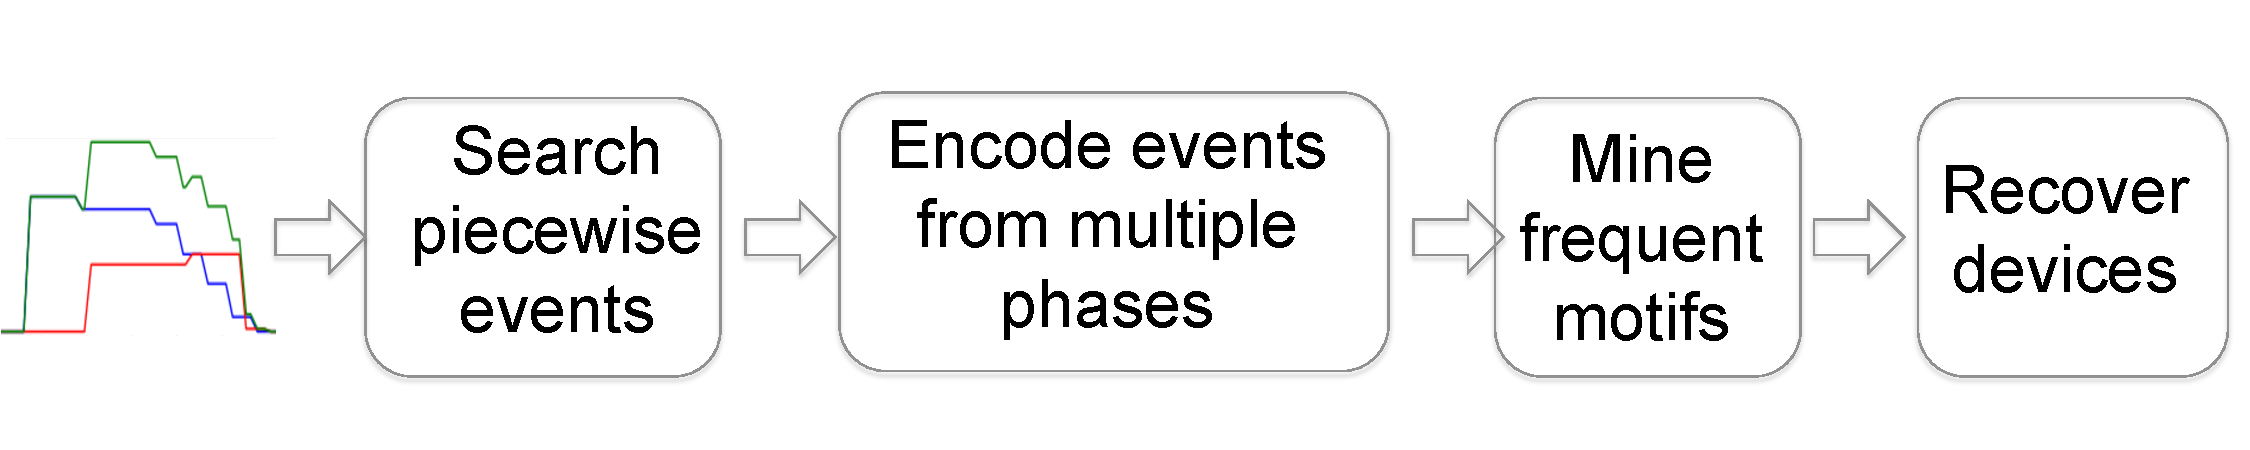
\includegraphics[width=0.7\textwidth]{multidisaggfig/multivariatePiecewiseMotifMining.pdf}
\caption{Multivariate Piecewise Motif Mining.}
\label{fig_multivariatePiecewiseMotifMining}
\end{figure}

\subsubsection{Piecewise Motif Mining}
Motif mining aims to uncover the repetitive patterns in time series data, and works best for discrete events. Piecewise motif mining is proposed 
for energy disaggregation to detect on/off events. 

\begin{definition}{\textbf{Piecewise Event}}
Given a time series diffs data $y_1, ...., y_{n'}$, where $\forall$ $|y_i| < \eta$. 
A piecewise event is the sum of these $n'$ number of diffs data, $e= \sum_{i=1}^{n'} y_i$. 
\end{definition}
Each piecewise event corresponds to an on/off event of an electric device. 
The value of $\eta$ is the noise range of each device, 
which is usually less than the 10\% of $|e|$.  

\textbf{Piecewise Events Search from Multiple Phases} \\
The majority of electrical devices which draw power from multiple phases consume larger amounts of power than electrical devices which connect to single phase. 
To disaggregate such a device, we need to 
discover specific on/off events features to separate them. 
%on/off events which are yielded by this single device from two-phase or three-phase aggregated data. 
Generally such an electrical device draws power from multiple phases synchronously 
and constructs a  pattern. 
Some devices may consume equal power from both phases all the time,  and so their power consumption patterns from both phases keep the same.
Other devices may show different power usage patterns when drawing power from two phases. 
%The power consumption from both phases may be exactly synchronized and keep the same all the time. 
%Either, the power consumption drawn from a single device differs much. 
\begin{algorithm}
\caption{Search Synchronized Events from Two-phase Aggregated Diffs Data}
\label{alg_synchronizeEvents}
\begin{algorithmic}[1]
\REQUIRE $2$-phases aggregated diffs data $y_k=y_1^{(k)}, ..., y_n^{(k)}$ and $k=1,2$, %each device's power levels and standard deviation $P_m$, $P_m^{std}$, 
big power consumption threshold $\theta$
%\ENSURE $y = x^n$
\FOR{$i=0: n-1$}
\IF { $|y_i^{(1)}| > \theta$}
\FOR{$j=i-5, i+5$}
\IF{ $|y_j^{(1)}| \in [ |y_j^{(2)}| * 0.8, |y_j^{(2)}| *1.2]$}
\STATE $e_i^{(1)}= e_i^{(1)} + y_j^{(1)}$
\STATE $e_i^{(2)}= e_i^{(2)} + y_j^{(2)}$
\ENDIF
\ENDFOR
\STATE $e_i = e_i^{(1)} +e_i^{(2)}$
\ENDIF
\ENDFOR
\RETURN $e_1, ..., e_i, ..., e_{n'}, \forall e_i > 2*\theta$
\end{algorithmic}
\end{algorithm}
Algorithm~\ref{alg_synchronizeEvents} describes how synchronized events from two phases are revealed.  
This input include the two-phase aggregated diffs data and big power consumption threshold $\theta$. 
This threshold guarantees we only discover big power consumption devices. 
We review the phase-1 diffs data. 
If any absolute value $|y_i^{(1)}|$ is greater than $\theta$, 
both previous and posterior five diffs data points from time $i$ are checked. 
For these 10 points values, 
at each time $j$, if the difference between phase-1 $y_i^{(1)}$ and phase-2 $y_i^{(2)}$ is in the range of $0.2*|y_i^{(1)}|$,  
we assert that the diffs data points from these two phases are relatively the same and synchronized. 
The synchronization implies that 
these two identical amounts power consumption comes from a single device. 
Therefore we sum the synchronized power level diffs data and compute the power consumption at time $i$ as $e_i$.  
When $e_i>0$ that denotes an on event, and $e_i<0$ means an off event for a certain device.

Next we transfer these two-phase diffs data into 
an ordered on/off event list $e_1, ..., e_{n'}$,
then we apply motif mining to this events list. 
By matching the devices which consume power greater than $2*\theta$, 
we can separate all devices which draw equal amount of power from two phases.  
%Since we already know the power levels of each device, 
%we just choose those devices which include power levels bigger than $2*\theta$. 
%By applying motif mining, 
%we can separate all devices which consume two-phase power greater than $\theta$ equally. 
%For dataset Study10, we set $\theta=500W$. 
%This approach helps us to discover two devices waterHeater2 and heatingIndoor. 
%All of the on/off events of these two devices are found out. 

\subsubsection{Encoding Events From Multiple Phases}
After deleting all the synchronized events from phase-1 and phase-2, 
we apply multivariate piecewise motif mining to the remaining phase-1 and phase-2 diffs data, 
to detect devices which consume large amounts of power 
and draw power from two phases synchronously yet unequally. 
There are different power drawing patterns from these two phases.  
We encode these two-phase diffs data, which occur at the same time, as a new event $e$. 
Figure \ref{fig_eventEncoding} gives an example of how the events from two-phase circuits
are encoded. 
We extract an event which consumes power greater than $\theta$, 
then we check five more data points before and after it. 
The values of the 11 data points relevant to this event in Main1.diff are [0, 0, -18, 18, 1093, 1830, -196, -68, -37, -36, 0]. 
The concurrent events listed in Main2.diff are [0, 0, 0, 18, 9, 1946, 440, -51,-36,-36,0]. 
Since the events at the peak occur in the two phases as $(1830, 1946)$, 
and the difference of these two powers $1946-1830=116$ is in the $0.2*1830$ range, 
we consider that these two changes may come from a single device. 
When looking for insight into these two vectors, 
we observe that the sum of the changes of phase 1 is 2604W, and the sum of the changes of phase 2 is 2290W. 
They are in the same range, i.e. $2604*0.8 < 2290$. 
Therefore, we declare that the power changes from these two phases definitely come from a single device. 
We select two of these values and encode them as $e_{1'}=(1093, 9)$, $e_{2'}= (1830, 1946)$
\begin{figure}[h]
\centering
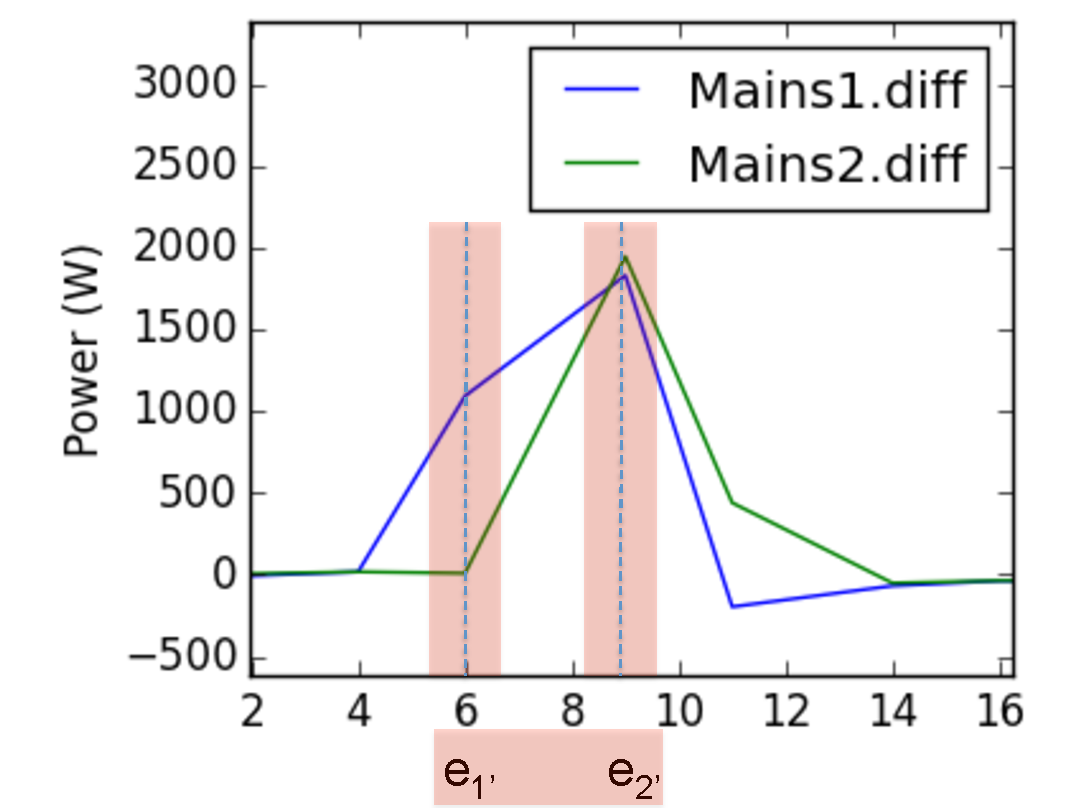
\includegraphics[width=0.5\textwidth]{multidisaggfig/synchronizeDifferentEventEncoding.pdf}
\caption{Encoding Events from Multiple Phases.}
\label{fig_eventEncoding}
\end{figure}

The piecewise events for this single device are $e= [e_{1'}, e_{2'}]$. 
Applying frequent motif mining, 
we separate this large power consumption device which draw power from two phases unequally. 




